\documentclass[10pt, a4paper, twocolumn]{jarticle}
%\documentclass[10pt, a4paper, twocolumn, uplatex]{jsarticle}
\usepackage{proceeding_bachelor}
\usepackage{tabularx}
\usepackage{booktabs}
\usepackage{multirow}
\usepackage{cite}
\usepackage{amsmath, amssymb}

% Title info. ======================================
\title{適応的PolyDice-1 Lossの提案と\\
医療画像セグメンテーションへの応用}

%%%%% 著者 %%%%%
\author{廣池 友哉}

%%%% 学籍番号 %%%%
\studentid{M243422}

%%%% 所属 %%%%
\affiliation{広島大学 大学院先進理工系科学研究科 情報科学プログラム}

%%%% 年度を書き換える %%%%
\proceedingname{2025年度修士論文中間発表予稿}

%%%% 卒論発表の日付を書く %%%%
\date{2025/9/19}


\begin{document}
%%%%%%%%%%%%% Header and Title %%%%%%%%%%%%%
\maketitle


%%% Please write your body text from here %%
\section{はじめに}
修士論文中間発表予稿の様式サンプルです.


発表予稿を\TeX{}で作成する場合は,
スタイルファイル\verb+proceedings_bachelor.sty+を利用してください.


その他の方法で発表予稿を作成する場合は,この様式を参考にしてください.


ただし,研究分野で特有の書式がある場合には,その様式に従ってください.


\section{数式の記述}
数式の記述例を次に示します.


本研究では,前節での調査結果から,光源スペクトルの周波数成分に基づいて波長サンプル組数を決定する.
すなわち,光源スペクトルをフーリエ変換した高周波数成分を重み付け加算した値を用いて
波長サンプル組数$S$を,次式により決定する.
%
\begin{equation}
S = a\sum_{i=0}^{n}F(i)g(i)+c
\end{equation}
%
ここで,$a$は重み付け加算した高周波成分に対する寄与係数,
$c$は最小波長サンプリング組数,
$F(i)$は第$i$調波成分の値,$n$は最大高周波,
$g(i)$は高周波成分に対する重み関数であり,次式とする.
%
\begin{equation}
g(i) = {\left(\frac{i}{b}\right)}^\gamma
\end{equation}
%
ここで,$b$は重み付け関数の調整係数,$\gamma$は重み付け関数べき乗係数である.
本研究では,前節での調査結果に基づき$a=2.1$,$b=100$,$c=5$,$\gamma=0.25$に設定した.
\newpage

\section{図表について}
\subsection{図の挿入}
図の使用例を次に示します.
\newline

Dice Lossは予測画像と正解画像との類似度を測るDice Indexに基づいて定義される.
$W \times H$(pixel)のモデルの予測画像を$\hat{\mathbf{y}} \in \mathbb R ^ {W \times H}$,
その画像に対する正解画像を$\mathbf{y} \in \mathbb R ^ {W \times H}$とすると,
Dice Lossは下記の式で示される.

\begin{equation}
  \mathcal{L}_{\text{Dice}}(\hat{\mathbf{y}}, \mathbf{y}) = 1 - \frac{2 \sum_{i=1}^{W} \sum_{j=1}^{H} \hat{y}_{ij} y_{ij}}{\hat{y_{ij}} ^ 2 + y_{ij} ^ 2}
\end{equation}


東広島キャンパスでは,図\ref{fig:campus}に示すように,
初夏にはアメリカ楓の美しい並木が緑に輝く.
%
\begin{figure}[t]
	\begin{center}
		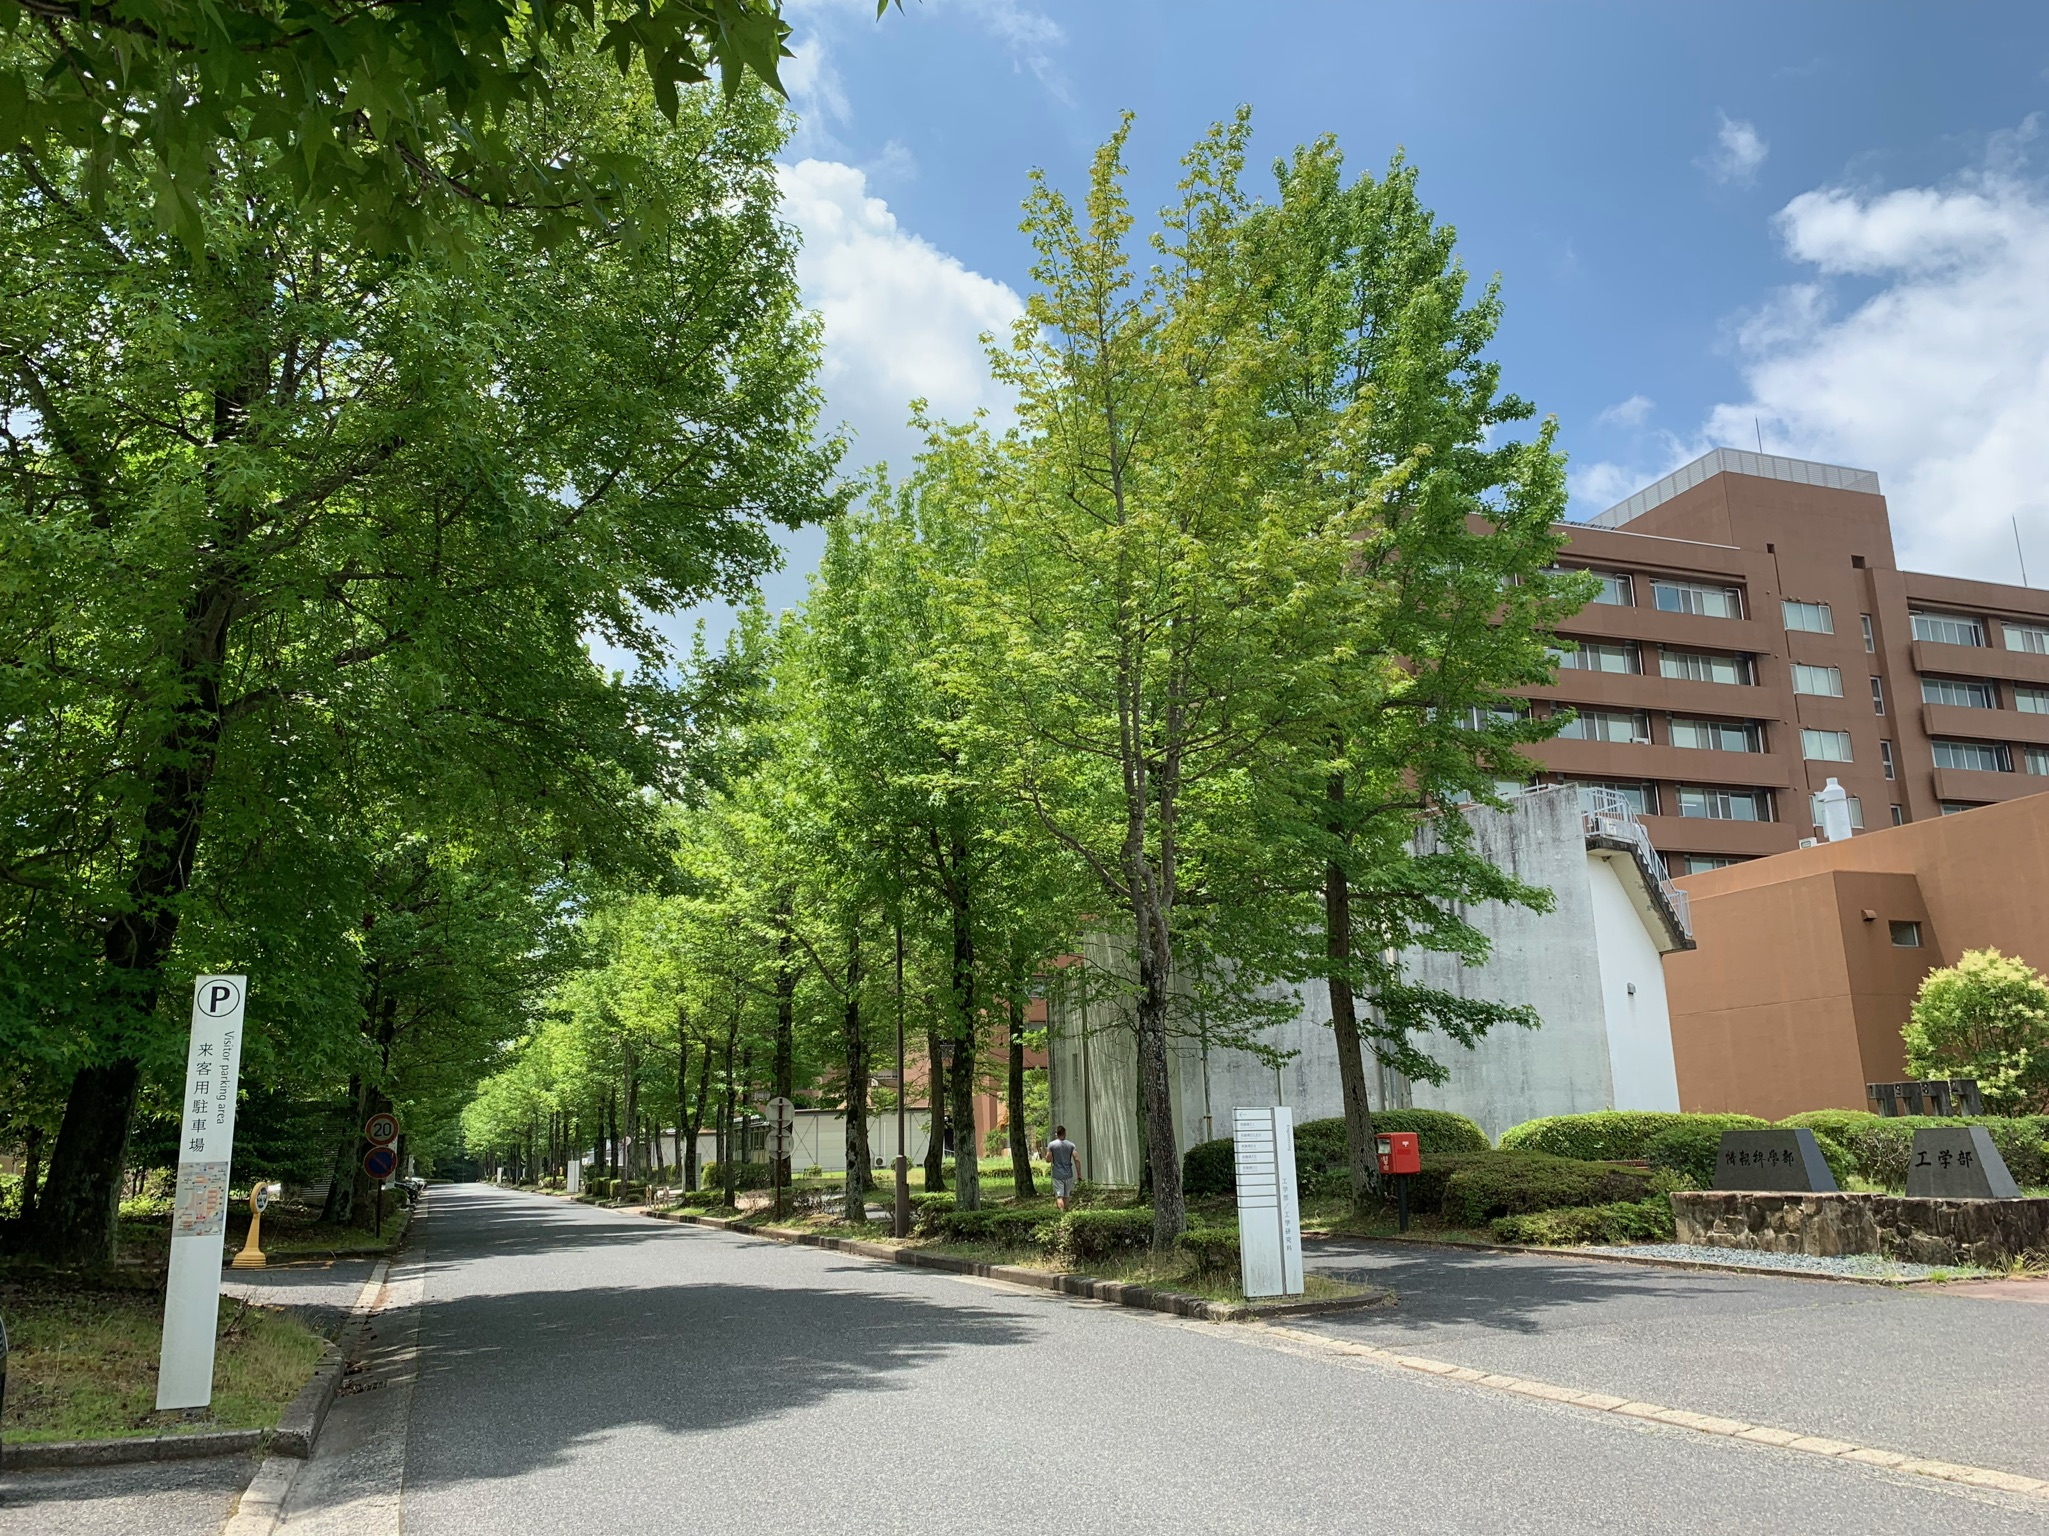
\includegraphics[width=0.95\hsize]{figure/campus.jpg}
	\end{center}
	\vspace{-12pt} %図とキャプションとの間隔調整
	\caption{東広島キャンパスのアメリカ楓並木}
	\label{fig:campus}
\end{figure}
%
\newline

Minkowski Islandは4つのMinkowski Sausage (Quadratic type 2 curve) を
正方形状に配置したフラクタル図形である(図\ref{fig:fractal}参照).
%
\begin{figure}[b]
	\begin{center}
		
\includegraphics[scale=1]{figure/fractal.pdf}
	\end{center}
	\vspace{-12pt} %図とキャプションとの間隔調整
	\caption{Minkowski Island}
	\label{fig:fractal}
\end{figure}
%
\newpage

\subsection{表の作成}
表の記入例を次に示します.

コースティックフォトンマップには,光源から放出されたフォトンが拡散反射面に到達する前に,
1回以上鏡面反射あるいは透過したフォトンの情報が格納される.
すなわち,表\ref{tab:path_notation}に示す表記法を用いれば,
{\tt LS+D}の経路をたどったフォトンの位置,放射束,入射方向が記録される.
%
\begin{table}[t]
  \begin{center}
  \caption{光の経路の表記法}
  \label{tab:path_notation}
  \begin{tabular}{l l | l l} \toprule
    {\tt L} & 光源 & {\tt (k)+} & {\tt k}が1回かそれ以上起きる \\ 
    {\tt E} & 視点 & {\tt (k)*} & {\tt k}が0回かそれ以上起きる \\
    {\tt S} & 鏡面反射 & {\tt (k)?} & {\tt k}が0回か1回起きる \\ 
    {\tt D} & 拡散反射 & {\tt (k|k')} & {\tt k}あるいは{\tt k'}が起きる \\ \bottomrule
  \end{tabular}
  \end{center}
\end{table}
%
\newline

\section{文献引用}
文献引用の例を次に示します.
\newline

レンダリング方程式(rendering equation)~\cite{kajiya1986rendering}は,算出すべき放射輝度$L$が式の両辺に表れた積分方程式となっている.

フォトンマッピング法~\cite{jensen2001realistic}では2段階のレイトレーシングを行うことによりレンダリング方程式を解く.


\section{まとめ}
修士論文中間発表予稿の様式を示しました.

%%%%% 参考文献(BibTeXを使う場合) %%%%%
\bibliographystyle{bibstyle} % bstファイルを設定
\bibliography{references} % bibファイルを読み込み

%%%%% 参考文献(直接書く場合) %%%%%
% \begin{thebibliography}{9} %\footnotesize
    % \bibitem{kajiya1986rendering}
    % J.~T. Kajiya,
    % \newblock ``The rendering equation,''
    % \newblock in {\em Proceedings of the 13th Annual Conference on Computer
    %   Graphics and Interactive Techniques}, pp. 143--150, 1986.
    
    % \bibitem{jensen2001realistic}
    % H.~W. Jensen,
    % \newblock {\em Realistic image synthesis using photon mapping}, vol. 364,
    % \newblock Ak Peters Natick, 2001.
% \end{thebibliography}

\end{document}